\documentclass[12pt,a4paper,twoside]{article}
\usepackage{labor}
\begin{document}

%fill for cover and header creation
\newcommand\laboratorynumber{2}
\title{Erneuerbare Energien}
\newcommand\supervisor{Ditlbacher, Harald}
\newcommand\groupnumber{42}

\newcommand\participantonelastname{Eisner}
\newcommand\participantonefirstname{Nico}
\newcommand\participantoneid{12214121}
\newcommand\participanttwolastname{Waldl}
\newcommand\participanttwofirstname{Philip}
\newcommand\participanttwoid{12214120}
\author{\participantonelastname \ \& \participanttwolastname}

\newcommand\degreeid{UB 033 678}
\newcommand\semester{23WS}
\date{10.11.2023}

%select correct course title
%\newcommand\coursetitle{Einführung in die \\ physikalischen Messmethoden}
%\newcommand\coursetitle{Laborübungen 1: \\ Mechanik und Wärme}
\newcommand\coursetitle{Laborübungen 2: \\ Elektrizität, Magnetismus, Optik}
%\newcommand\coursetitle{Fortgeschrittenen Praktikum 1: \\ Technische Physik}
%\newcommand\coursetitle{Fortgeschrittenen Praktikum 2: \\ Allgemeine Physik}

%\begin{titlepage}
   \begin{center}
       \begin{figure}[H]
            \begin{minipage}[h]{30mm}
                \centerline{
\includegraphics[height=15mm]{cover_nudes/tugraz.png}}
            \end{minipage}
            \hfill
            \begin{minipage}[h]{30mm}
                \centerline{
\includegraphics[height=15mm]{cover_nudes/nawi_graz.png}}
            \end{minipage}
            \hfill
            \begin{minipage}[h]{30mm}
                \centerline{
\includegraphics[height=15mm]{cover_nudes/uni-graz.png}}
            \end{minipage}
        \end{figure}
        
        \large{\emph{Institut für Experimentalphysik der Technischen Universität Graz \\
        \& Institut für Physik der Universität Graz}} \\
        \vspace{5mm}
        
        {\Huge \textbf{\coursetitle}}
        \vspace{5mm}
        
        {\huge \laboratorynumber: \thetitle}
    \end{center}
    
    \vfill
    
    \begin{table}[H]
        \LARGE
        \centering
        \begin{tabular}{r l}
            Betreuer:       & \supervisor \\
            Gruppennummer:  & \groupnumber \\
            \\
            Name:           & \participantonelastname, \participantonefirstname \\
            Matrikelnummer: & \participantoneid \\
            Name:           & \participanttwolastname, \participanttwofirstname \\
            Matrikelnummer: & \participanttwoid \\
            \\
            Kennzahl:       & \degreeid \\
            Datum:          & \semester \ | \thedate
        \end{tabular}
    \end{table}
    \vspace{4cm}
\end{titlepage}
\clearpage
\setcounter{page}{1}

%\maketitle %short title alternative


\includepdf[pages={1}]{../Deckblätter/Deckblatt_Erneuerbare_Energie.pdf}

\tableofcontents
\newpage

\section{Aufgabenstellung} %jo beschreibn wos gmocht host ------------------------------
Der Versuch Erneuerbare Energien besteht aus mehreren verschiedenen Teilen, wo mit unterschiedlichen Methoden zur Energieerzeugung gearbeitet wird. 

\subsection{Photovoltaik}
Im ersten Teilversuch gilt es mithilfe zweier Solarmodule und einer Lampe, welche als Sonne dient, verschiedene Schaltungstypen zu Testen und die Leerlaufspannung und den Kurzschlussstrom zu ermitteln. \\
Im weiteren Teil wird das selbe für unterschiedliche Abstände zur Lichtquelle wiederholt. 
\subsection{Brennstoffzelle}
Bei dem Teil der Brennstoffzelle wird an die Zelle Spannung angelegt und gemessen, ab welcher Spannung sich die Gastanks zu füllen beginnen. \\
Im zweiten Teil mit der Brennstoffzelle gilt es den Wirkungsgrad zu bestimmen. Dazu wird die Volumensänderung pro Zeit im Gastank gemessen. \\
Beim dritten Teil wird die Kennlinie der Brennstoffzelle ermittelt. Durch schrittweises verringern des Widerstandes an einem Potentiometer lässt sich die Spannung und der Strom messen und daraus die Leistung berechnen. 

\subsection{Windmaschine}
Im ersten Teil wird die Windmaschine vor ein Windrad gestellt und mit unterschiedlichen Eingangsspannungen wird die Leerlaufspannung am Windrad gemessen. 
Anschließend wird die Eingangsspannungen an der Windmaschine fixiert und das Windrad in gewissen Abständen davon entfernt und erneut die Leerlaufspannung gemessen. \\
Im zweiten Teil wird Beobachtet, was bei einzelnen Extremfällen passiert. Dazu wird der Luftstrom abbrupt gestoppt und die Leerlaufspannung am Windrad wird gemessen. 
Anschließend wird der Luftstrom abbrupt gestartet und es wird erneut die Leerlaufspannung gemessen. die beiden Extremfälle werden anschließend mit einer Kapazität zwischen Windrad und Multimeter wiederholt. 

\subsection{Speicherung der Energie}
Durch ein Windrad wird Energie erzeugt, welche genutzt wird um an der Brennstoffzelle Elektrolyse zu betreiben. Hierbei wird die Energie als chemisches Potential gespeichert. 
\\
\\
Alle Informationen und Methodiken wurden uns von der Technischen Universität bereitgestellt \cite{teachcenter2}. 



\section{Voraussetzungen \& Grundlagen} %Grundlagen erklären, Formeln mit erklärung

    \begin{equation}
        \label{eq:Müll}
        \centerline{$M=\frac{muell}{malle}$}
    \end{equation}

\section{Versuchsanordnung} %mit skizze kurz beschreiben ------------------------------

    \begin{figure}[H]
        \centering
        %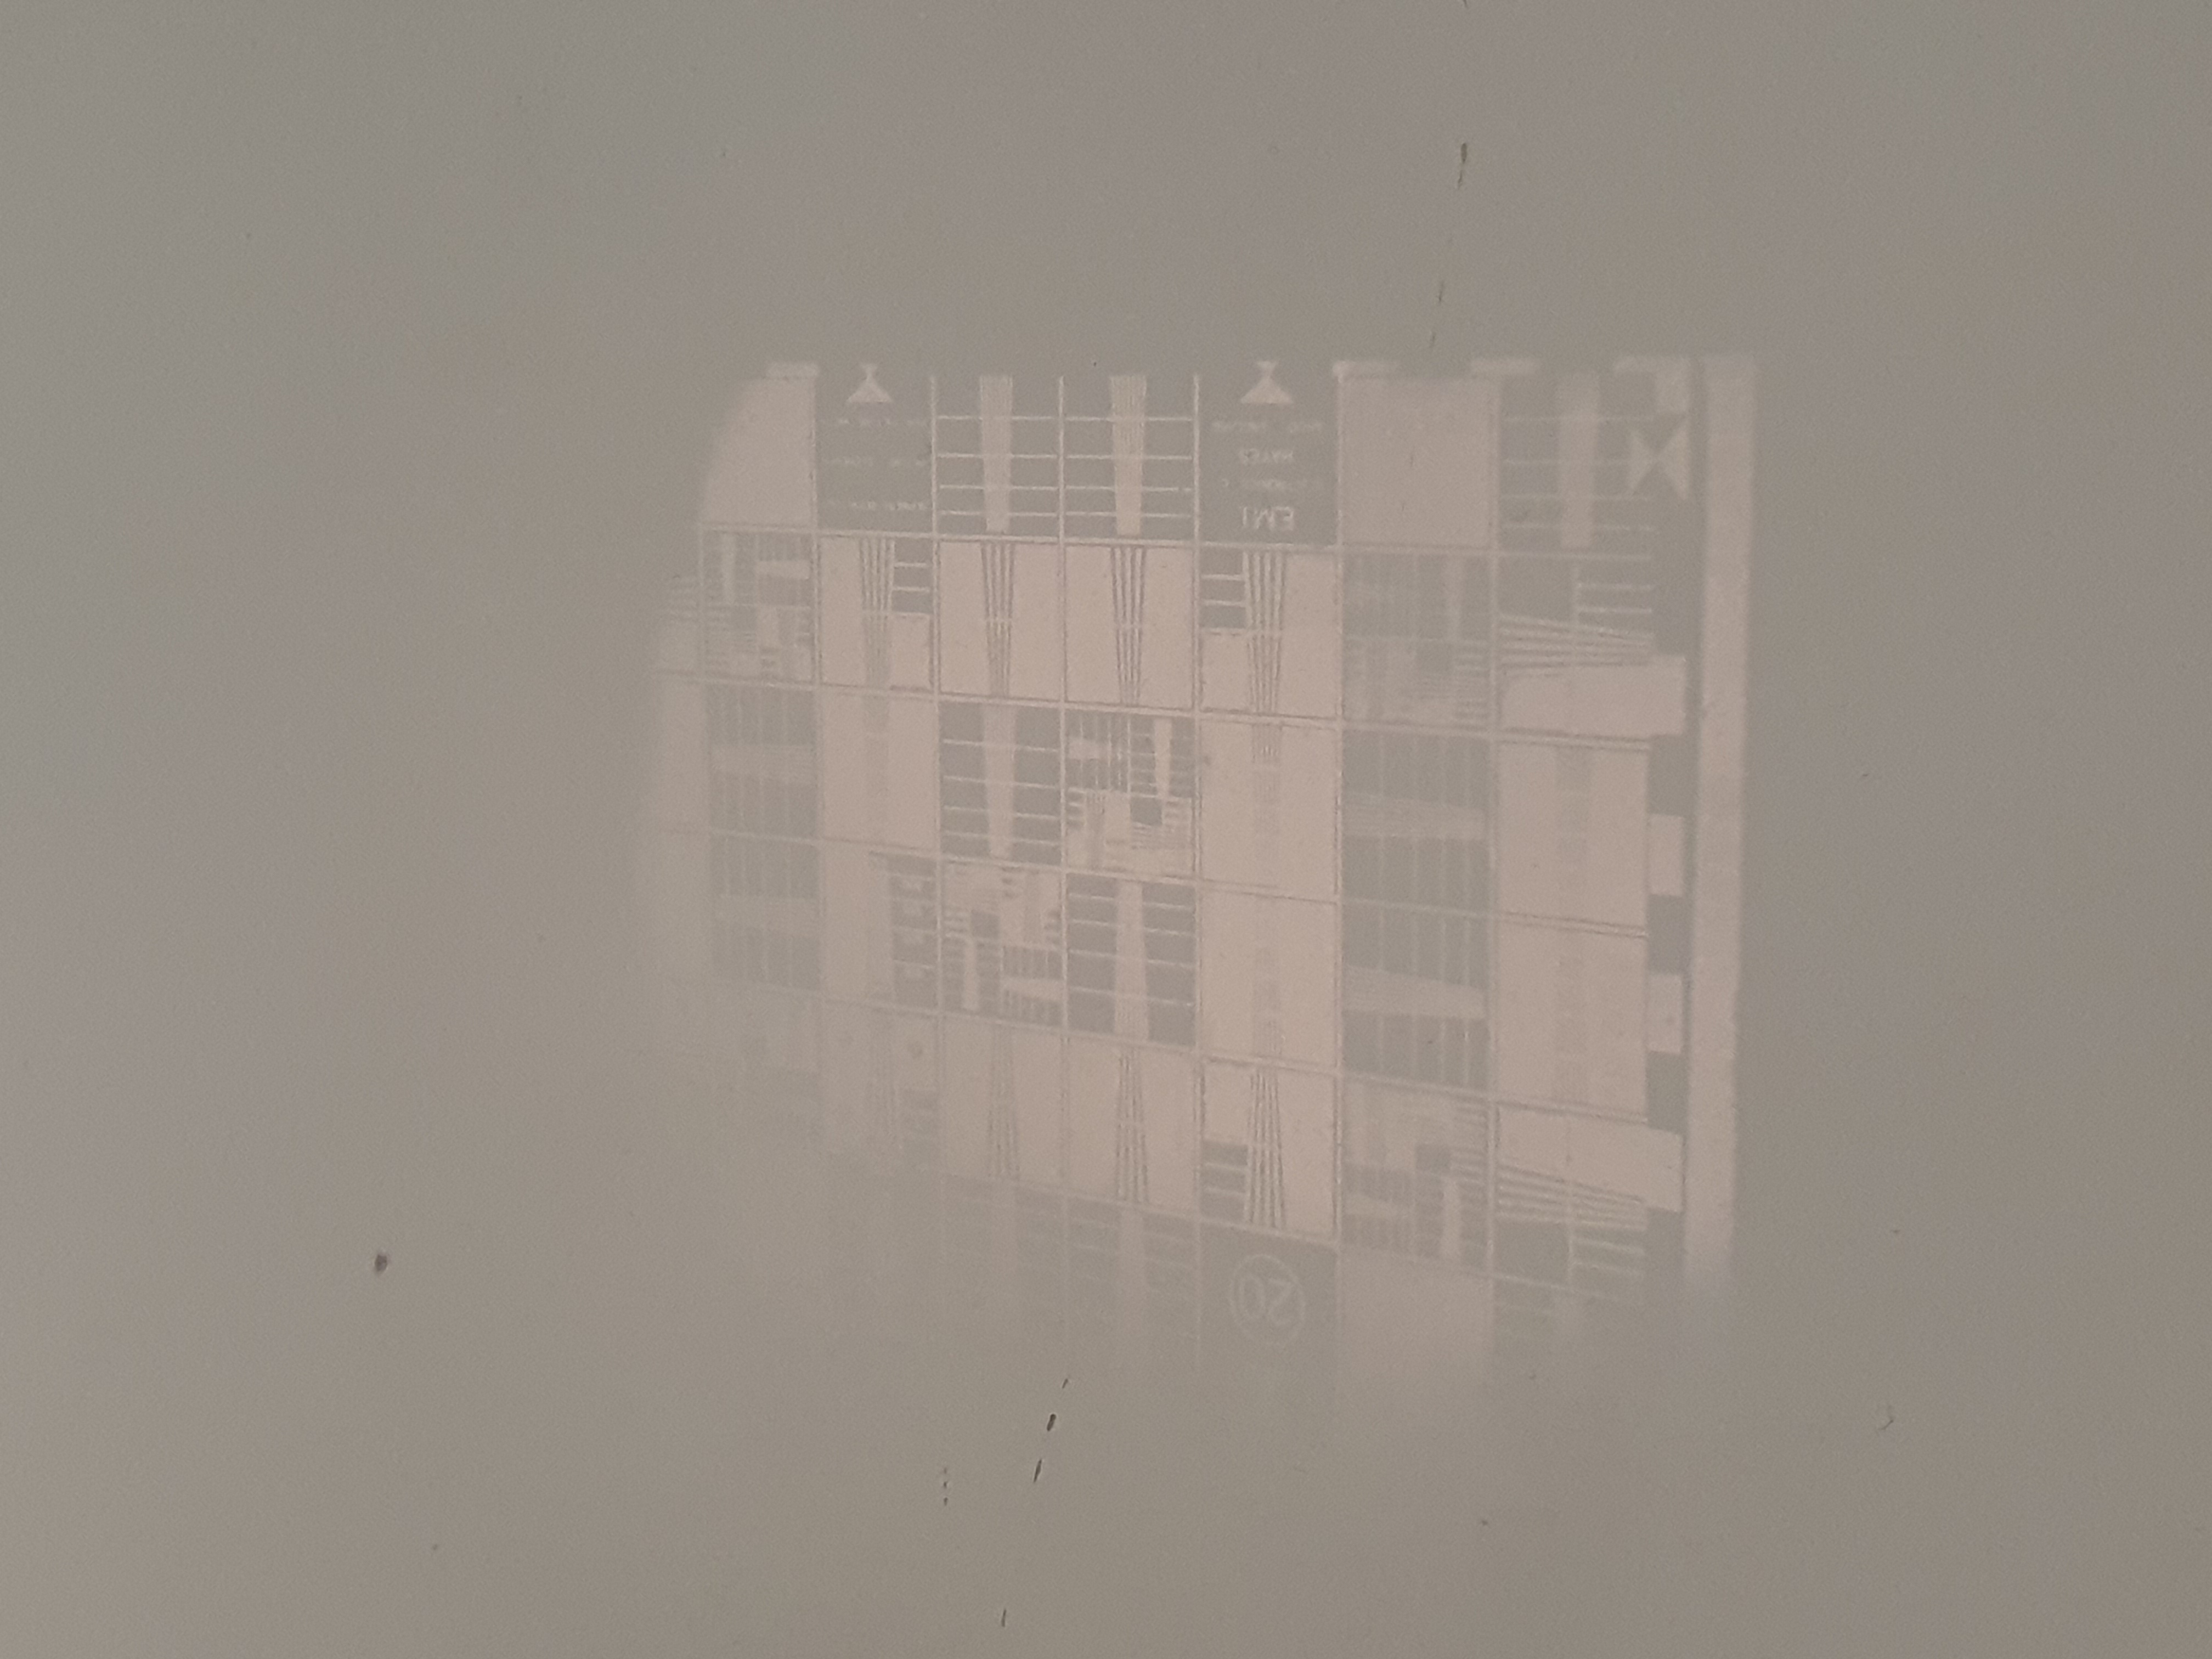
\includegraphics[width=0.6\linewidth, angle=-90]{nudes/bild.jpg}
        \caption{müll}
        \label{fig:müllbild}
    \end{figure}

\section{Geräteliste} %jo holt a listn ------------------------------

    \begin{table}[H]
        \centering
        \caption{Im Versuch verwendete Geräte und Utensilien.}
        \label{tab:geraete}
        \begin{tabular}{| l | l | l | l |}
            \hline
            Gerät   & Typ   & Gerätenummer  & Unsicherheit \\
            \hline
        \end{tabular}
    \end{table}


\section{Versuchsdurchführung \& Messergebnisse} %nachvollziehbar und klar dargestellt ------------------------------


\section{Auswertung und Unsicherheitsanalyse} %Nicht nur zahlen angeben ------------------------------

In der Auswertung werden zur erhöhten Genauigkeit durchgehend ungerundete Werte bis zu den Endergebnissen verwendet und nur zur Darstellung gerundet. \\
Zur Berechnung der Unsicherheiten wird, wenn nicht anders angegeben, die Größtunsicherheitsmethode verwendet.


\section{Diskussion} %diskussion der Unsicherheiten und Ergebnisse und evtl. verlgeich mit Literatur ------------------------------


\section{Zusammenfassung} %klare, übersichtliche vollständige beantwortung der Aufgabenstellung ------------------------------


\printbibliography[heading=bibintoc]
\end{document}
